\documentclass[preprint,12pt, a4paper]{elsarticle}

\usepackage{amssymb}

\usepackage{amsthm}
\usepackage{mathtools}

\usepackage{lineno}

\usepackage{float}

\usepackage{todonotes} 
\usepackage{url}

\restylefloat{table}

\newcommand{\eg}{{\emph{e.g.\/}}}
\newcommand{\ie}{{\emph{i.e.\/}}}
\newcommand{\ket}[1]{\ensuremath{|#1\rangle}}
\newcommand{\bra}[1]{\ensuremath{\langle#1|}}
\newcommand{\ketbra}[2]{\ensuremath{\ket{#1}\bra{#2}}}
\newcommand{\proj}[1]{\ensuremath{\ketbra{#1}{#1}}}
\newcommand{\braket}[2]{\ensuremath{\langle{#1}|{#2}\rangle}}
\newcommand{\floor}[1]{\ensuremath{\lfloor #1 \rfloor}}
\newcommand{\complexity}[1]{\ensuremath{\mathbf{#1}}}
\newcommand{\new}[1]{ \textcolor{red}{#1} }
\newcommand{\1}{{\rm 1\hspace{-0.9mm}l}}
\newcommand{\Id}{{\rm 1\hspace{-0.9mm}l}}
\newcommand{\connected}{\sim}
\newcommand{\SPAN}{\mathrm{span}}
\newcommand{\Lrm}{\ensuremath{\mathrm{L}}}
\newcommand{\Urm}{\ensuremath{\mathrm{U}}}
\newcommand{\ee}{\ensuremath{\mathrm{e}}}
\newcommand{\dd}{\ensuremath{\mathrm{d}}}
\newcommand{\ii}{\ensuremath{\mathrm{i}}}
\newcommand{\EE}{\mathcal{E}}
\newcommand{\XX}{\mathcal{X}}
\newcommand{\MM}{\mathcal{M}}
\newcommand{\NN}{\mathcal{N}}
\newcommand{\DD}{\mathcal{D}}
\newcommand{\TT}{\mathcal{T}}
\newcommand{\PP}{\mathcal{P}}
\renewcommand{\SS}{\mathcal{S}}
\newcommand{\UU}{\mathcal{U}}
\newcommand{\HH}{\mathcal{H}}
\newcommand{\DU}{\mathcal{DU}}
\newcommand{\NOT}{\sigma_x}
\newcommand{\idop}[1][\XX]{\ensuremath{\1_{#1}}}
\newcommand{\diaguni}{\ensuremath{\mathcal{DU}}}
\newcommand{\diag}{\mathrm{diag}}
\newcommand{\tr}{\mathrm{tr}}
\journal{SoftwareX}


\usepackage{amsmath}
\newtheorem{theorem}{Theorem}
\newtheorem{proposition}{Proposition}
\newtheorem{remark}{Remark}
\newtheorem{scheme}{Scheme}
\newtheorem{lemma}{Lemma}

\begin{document}

\begin{frontmatter}

\title{PyQBench: a Python library for benchmarking gate-based quantum computers}

\author{Konrad Jałowiecki\corref{cor1}}
\ead{dexter2206@gmail.com}
\cortext[cor1]{Corresponding author}

\author{Paulina Lewandowska}
\author{Profesor Kierownik \L ukasz Pawela}

\address{Institute of Theoretical and Applied Informatics, Polish Academy
	of Sciences, Ba{\l}tycka 5, 44-100 Gliwice, Poland}

\begin{abstract}
We introduce PyQBench, an innovative open-source framework for benchmarking 
gate-based quantum computers. PyQBench can benchmark NISQ devices by verifying their capability of
discriminating between two von Neumann measurements. PyQBench offers a simplified, ready-to-use,
command line interface (CLI) for running benchmarks using a predefined parametrized Fourier
family of measurements. For more advanced scenarios, PyQBench offers a way of employing user-defined
measurements instead of predefined ones.

\end{abstract}

\begin{keyword}
%% keywords here, in the form: keyword \sep keyword
Quantum computing \sep
Benchmarking quantum computers \sep 
Discrimination of quantum measurements \sep 
Discrimination of von Neumann Measurements \sep
Open-source \sep
Python programming

%\PACS 03.67.−a \sep 03.67.Lx
		
\MSC 81P68

\end{keyword}

\end{frontmatter}

\section*{Required Metadata}
\label{}

\section*{Current code version}
\label{}

Ancillary data table required for subversion of the codebase. Kindly replace 
examples in right column with the correct information about your current code, 
and leave the left column as it is.

\begin{table}[H]
\begin{tabular}{|l|p{6.5cm}|p{6.5cm}|}
\hline
\textbf{Nr.} & \textbf{Code metadata description} & \textbf{Please fill in this 
column} \\
\hline
C1 & Current code version & For example v42 \\
\hline
C2 & Permanent link to code/repository used for this code version & For 
example: $https://github.com/mozart/mozart2$ \\
\hline
C3 & Code Ocean compute capsule & For example: 
$https://codeocean.com/2017/07/30/neurospeech-colon-an-open-source-software-for-parkinson-apos-s-speech-analysis/code$\\
\hline
C4 & Legal Code License   & List one of the approved licenses \\
\hline
C5 & Code versioning system used & For example svn, git, mercurial, etc. put 
none if none \\
\hline
C6 & Software code languages, tools, and services used & For example C++, 
python, r, MPI, OpenCL, etc. \\
\hline
C7 & Compilation requirements, operating environments \& dependencies & \\
\hline
C8 & If available Link to developer documentation/manual & For example: 
$http://mozart.github.io/documentation/$ \\
\hline
C9 & Support email for questions & \\
\hline
\end{tabular}
\caption{Code metadata (mandatory)}
\label{} 
\end{table}


\linenumbers

%% main text

The permanent link to code/repository or the zip archive should include the 
following requirements: 

README.txt and LICENSE.txt.

Source code in a src/ directory, not the root of the repository.

Tag corresponding with the version of the software that is reviewed.

Documentation in the repository in a docs/ directory, and/or READMEs, as 
appropriate.




\section{Motivation and significance}

Noisy intermediate-scale quantum
(NISQ)~\cite{preskill} devices are currently storming the market. We
have a selection of readily available quantum computers based on different
architectures. Historically, the first widely introduced quantum computing
architecture is D-Wave's quantum annealer~\cite{}. 

https://quantumcomputingreport.com/scorecards/qubit-technology/

Additional approaches to quantum computing are currently in development. For 
instance we have Ionq's computer based on ion traps and Xanadu's optical 
lattices. As they are in prototype versions no access to general public is 
provided. 

Next, we have computers implementing the gate model of quantum computation.
These are the best potentially developed machines, which can be thought
of as fully quantum computers, by which we understand that the qubits can be in
an entangled state. 

Currently one of the main providers of such architectures is Rigetti and its 
Quantum Cloud Services platform. The company has
released three generations of QPUs so far: Rigetti 8Q Agave, Rigetti 19Q Acorn
and Rigetti 16Q Aspen-1. The most recent one was deployed in November 2018 and
is a downgrade in terms of number of qubits compared to the previous 19 qubit
one. However, the new chip is reportedly much more robust to noise and the
proposed architecture is much easier to scale up. The new unit is supposed to
serve as a building block for a 128 qubit
system~\footnote{https://medium.com/rigetti/the-rigetti-128-qubit-chip-and-what-it-means-for-quantum-df757d1b71ea}.
As was the case for IBM, Rigetti also provides a \texttt{Python} library, 
\texttt{pyquil}~\cite{}, which enables easy access to the machine.

\todo[inline]{co napisac o tym Amazonie, czy nic ?}

\todo[inline]{rysunki architektur}

%
%\begin{figure}[h]
%	\centering 
%	
%	\includegraphics[width=0.9\linewidth]{aspen.png} 
%	\caption{?}
%	\label{fig:aspen}
%\end{figure}


Now the natural question arises: how to construct a good metric of the
computational power of such devices? 
Lately, there have emerged propositions from the scientific community on how to
benchmark such devices.

 First let us mention the work by Michielsen
\emph{et.al.}~\cite{michielsen2017benchmarking}. In there the authors study the
IBM-QE device. Their first test is the creation of the entangled state
$\frac{1}{\sqrt{2}} (\ket{01} - \ket{10})$. Next they implement a
two-qubit+two-qubit adder. Another test is an identity operation, realized by an
even number of CNOT operations. Their final test is a quantum error correction
scheme (is it possible with measurement-controlled-operations?). The final
conclusion is that, except for simple circuits, the device fails to return
correct results.

Another, recent approach is utilizing quantum communication protocols in testing
of quantum architectures~\cite{zhukov2019quantum}. Here, the authors decide to
utilize superdense coding and the BB84 quantum cryptography protocol as
benchmarks for the IBM Q devices. They utilize the mutual information of the
transferred bits as a figure of merit for the quantum computer.

Other approaches focus on generative model training. One of these
works~\cite{hamilton2018generative} is aimed at small architectures, up to 5
qubits. Another recently presented is much more
robust~\cite{benedetti2018generative}. The main drawback of both of them is the
level of complication.



The goal of this work is to introduce a new benchmark for Rigetti 
architecture...


\label{}
\todo[inline]{
	Introduce the scientific background and the motivation for developing the 
	software. - motywacje 
	
	Explain why the software is important, and describe the exact (scientific) 
	problem(s) it solves. - czemu ejst wazne, jakie problemy rozwiazuje 
	
	Indicate in what way the software has contributed (or how it will 
	contribute in the future) to the process of scientific discovery; if 
	available, this is to be supported by citing a research paper using the 
	software. - do czego sie to przyczyni w przyszlosci 
	
	Provide a description of the experimental setting (how does the user use 
	the software?). - w jaki sposób użytkownik korzysta z oprogramowania?
	
	Introduce related work in literature (cite or list algorithms used, other 
	software etc.). - inne oprogramowania i algorytmy }



\section{Software description}
\label{}
\todo[inline]{Describe the software in as much as is necessary to establish a 
vocabulary needed to explain its impact. }

We will first give a general overview of the structure of the code in 
Section~\ref{sec:sortware-architecture} and then provide additional details on 
the functionality of benchmark's schemes  in 
Section~\ref{sec:sortware-functionalities}.

\subsection{Software Architecture}\label{sec:sortware-architecture}
\label{}
\todo[inline]{
	Give a short overview of the overall software architecture; provide a 
	pictorial component overview or similar (if possible). If necessary provide 
	implementation details.}


\subsection{Software Functionalities}\label{sec:sortware-functionalities}
\todo[inline]{Present the major functionalities of the software.}

In the scope of this Paper, we aim at  exploring ideas revolving around quantum 
gate model-inspired computing devices, and assess their feasibility to 
benchmark a modern quantum architectures. The main idea that we have envisioned 
for this project is  introducing new concepts of benchmarks for NISQ devices 
benchmarking. This project aims to characterize the computing power and 
investigate possible practical applications of such devices having access by 
Amazon Braket. 





\subsubsection{Model specification}
The scenario assumes that Alice and Bob have access to an unknown measurement
device, a black box. Alice has hidden one of the two measurements, either $\PP$
or $\mathcal{Q}$, in the black box. Bob only has the information that the black box
performs one of these measurements. They want to determine an upper bound on the
probability of correct discrimination between $\PP$ and $\mathcal{Q}$. Moreover, they also want to
construct an optimal discrimination strategy to achieve the highest probability. Theoretical results were characterized in~\cite{puchala2018strategies}.



In this work, we will consider the problem of discrimination between von Neumann 
measurements. One of them on the computational basis, the second one on basis 
$U$, where $U$ is a unitary matrix. 
The scheme of discrimination can be divided into the following steps, which are 
illustrated in Fig.~\ref{fig:theoretical_scheme}.


\begin{figure}[h!]
	\centering
	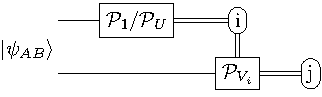
\includegraphics[scale=1.7]{pics/theoretical_scheme}
	\caption{Theoretical  scheme of discrimination  between von Neumann measurements $\PP_{U}$ and $\PP_\Id$. }
	\label{fig:theoretical_scheme}
\end{figure}

%\begin{figure}[h!]
%	\centering 
%	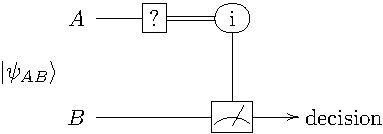
\includegraphics[width=0.9\linewidth]{gates1.pdf} 
%	\caption{A schematic representation of the setup for distinguishing
%		measurements by using entanglement. }
%	\label{fig:scheme}
%\end{figure}


\begin{enumerate}
	\item Alice and Bob share an entangled state $\ket{\psi_{0}}$ (discriminator) on systems 
	$A$ and $B$.
	\item Alice performs one of two known measurements (either $\PP_{\Id}$ or 
	$\PP_{U}$) on part $A$ of the input state  $\ket{\psi_{0}}$ and measures the system $A$.
	\item Alice performs the conditional binary measurement $\PP_{V_i}$ on the part 
	$B$ based on the output label $i$. 
	\item  Bob measures the system $B$ of the input state  $\ket{\psi_{0}}$ and 
	makes a decision based on the received label $j$. If $j=0$, then he decides 
	that the the black box contains $\PP_U$. Otherwise, he decides that the 
	black box contains $\PP_{\Id}$. 
\end{enumerate}  



\subsubsection{Quantum architecture's limits and practical solutions}



Let us take a closer look at the setup for distinguishing von Neumann 
measurements (see Fig.~\ref{fig:theoretical_scheme}). One of the components of 
this scheme is to perform a conditional binary measurement. 
Unfortunately, current NISQ devices do not allow for performing conditional 
binary measurements.
The only possible measurement performed on quantum architectures is the 
measurement in the computational basis. 
We  will present two possible methods providing a clever way to cross this 
obstacle. These will be two schemes of practical realization. 
The first method consists in using postselection while the second method 
consists in applying a controlled unitary. These methods are described below. 

\begin{scheme}(Postselection)



%\begin{figure}[h!]
%	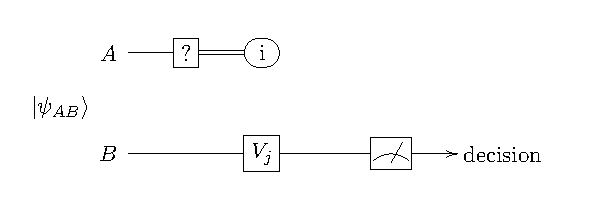
\includegraphics[scale=1.5]{onequbit.pdf}
%	\caption{A schematic representation of the setup for distinguishing
%		measurements using postselection.}
%	\label{postselection}
%\end{figure}






\begin{enumerate}
\item Alice and Bob prepare an entangled state $\ket{\psi_{0}}$ (discriminator) on systems 
$A$ and $B$.
\item Alice performs one of two quantum channels, either $\Phi_{\Id}$ or 
$\Phi_{U^\dagger}$,  on part $A$ of the input state  $\ket{\psi_{0}}$.
\item Alice measures part $A$ of the input state  $\ket{\psi_{0}}$ and 
receives an output label $i$.
\item  
Based on Holevo--Helstrom theorem, Bob performs a conditional binary 
measurement	$\PP_{V_j}$ and implements the unitary channel 	$\Phi_{V_j^\dagger}$ on part $B$.
\item To calculate the probability of correct discrimination, they include just those cases for which $i = j$.
\item Bob measures part $B$ of the input state  $\ket{\psi_{0}}$ and makes a
decision based on received label $j$. If $i=j=0$, then he decides that the 
black box contains $\PP_U$. Otherwise, he decides that the black box contains
$\PP_{\Id}$.
\end{enumerate}


The schematic representation of this setup is depicted in 
Fig.~\ref{fig:postsellection}.     

\begin{figure}[h!]
	\centering 
	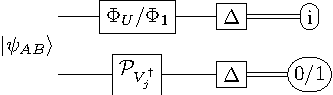
\includegraphics[scale=1.7]{pics/postselection} 
	
	\caption{ A schematic representation of the setup for distinguishing
		measurements using postselection. 
	}\label{fig:postsellection}
\end{figure}  

Due to the fact that the measurement result is nondeterministic, we are forced to consider the following circuits
in the postselection procedure
\begin{equation}
\begin{split}
(\Phi_{U^\dagger}, \Phi_{V_k^\dagger}, i, j) \\ 
(\Phi_{\Id}, \Phi_{V_k^\dagger}, i, j)
\end{split}
\end{equation}
where $k=\{0,1\}, i=\{0,1\}$ and $ j=\{0,1\}$. 
The optimal probability of correct discrimination between $\PP_{U} $ and $\PP_\Id$ is as follows.
		\begin{equation}
		p = \frac{\#(\Phi_{U^\dagger}, \Phi_{V_i^\dagger},i,0) + \#(\Phi_\Id, \Phi_{V_i^\dagger},i,1)}{\#(\Phi_{U^\dagger}, \Phi_{V_i^\dagger},i,j) + \#(\Phi_\Id, \Phi_{V_i^\dagger},i,j)}, 
		\end{equation}
where $i=\{0,1\}$ and $ j=\{0,1\}$. 

\end{scheme}


\begin{scheme}(By using controlled unitary)
	


\begin{enumerate}
\item Alice and Bob prepare an entangled state $\ket{\psi_{0}}$ on 
systems $A$ and $B$.
\item Alice performs one of two quantum channels, either $\Phi_{\Id}$ or
$\Phi_{U^\dagger}$,  on part $A$ of the input state  $\ket{\psi_{0}}$.
\item Alice and Bob implement  direct sum of unitary channels $\Phi_{V_0^\dagger} \oplus \Phi_{V_1^\dagger}$ obtained from 
Holevo--Helstrom theorem.	
\item Alice and Bob prepare the measurement $\Delta$ in computational basis on 
their systems.
\item Bob makes a decision based on received label $j$. If $j=0$, then he
decides that the the black box contains $\PP_U$. Otherwise, he decides that the
black box contains $\PP_{\Id}$.
\end{enumerate}

The schematic representation of this setup is depicted in 
Fig.~\ref{fig:controlled}.     
\begin{figure}[h!]
	\centering 
	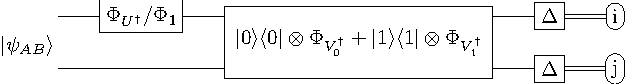
\includegraphics[scale=1.5]{pics/controlled_unitary} 
	
	\caption{ A schematic representation of the setup for distinguishing
		measurements using controlled unitary gate. 
	}\label{fig:controlled}
\end{figure} 


Here, we consider the following circuits
by using controlled unitary
\begin{equation}
\begin{split}
(\Phi_{U^\dagger}, \Phi_{V_0^\dagger} \oplus \Phi_{V_1^\dagger}, i, j) \\ 
(\Phi_{\Id},  \Phi_{V_0^\dagger} \oplus \Phi_{V_1^\dagger}, i, j)
\end{split}
\end{equation}
where $i=\{0,1\}$ and $ j=\{0,1\}$. 
Then, the optimal probability of correct discrimination between $\PP_{U} $ and $\PP_\Id$ is as follows.
\begin{equation}
p = \frac{\#(\Phi_{U^\dagger},\Phi_{V_0^\dagger} \oplus \Phi_{V_1^\dagger},i,0) + \#(\Phi_\Id,\Phi_{V_0^\dagger} \oplus \Phi_{V_1^\dagger},i,1) }{\#(\Phi_{U^\dagger},\Phi_{V_0^\dagger} \oplus \Phi_{V_1^\dagger},i,j) + \#(\Phi_\Id,\Phi_{V_0^\dagger} \oplus \Phi_{V_1^\dagger},i,j)}
\end{equation}
where $i=\{0,1\}$ and $ j=\{0,1\}$. 
\end{scheme}




\subsubsection{Mathematical preliminaries}



Let $M_{d_1,d_2}$ be the set of all matrices of dimension $d_1 \times d_2$ over
the field $\mathbb{C}$. For  simplicity, square matrices will be denoted by
$M_d$.  
%The subset of $M_d$ consisting of Hermitian matrices of dimension $d$
%will  be  denoted  by $\HH_d$,  while  the  set  of  positive semidefinite
%matrices of dimension $d$ by $\HH_d^+$. 
The set of quantum states, that is
positive semidefinite operators having trace equal to one, will be denoted
$\Omega_d$. 
 The subset of $M_d$ consisting of unitary matrices will be denoted
by $\UU_d$, while its subgroup of diagonal unitary operators will be denoted by
$\DD \UU_d$. 
	An operator $A = \left( a_{i,j}\right)_{i,j} \in M_d$ is said to be a stochastic matrix if $a_{i,j} \ge 0$   and $\sum_{i} a_{i,j} = 1$, whereas an operator $A = \left( a_{i,j}\right)_{i,j} \in M_d$ is said to be a double stochastic matrix if $A$ is a stochastic matrix and $\sum_{j} a_{i,j} = 1$.


 We will also need a linear mapping transforming $M_{d_1}$ into
$M_{d_2}$, which will be denoted 
\begin{equation}
\Phi: M_{d_1 } \rightarrow M_{d_2}.
\end{equation} 
There
exists a bijection between the set of linear mappings $\Phi$ and the set of matrices $M_{d_1d_2}$,  known as the Choi-Jamio{\l}kowski isomorphism. 
For a given linear mapping $\Phi$ the corresponding Choi operator $\mathcal{J}(\Phi)$ is explicitly written as 
\begin{equation}
\mathcal{J}(\Phi) \coloneqq \sum_{i,j=0}^{d- 1} \Phi(\ketbra{i}{j}) \otimes \ketbra{i}{j}. \end{equation}
We introduce a special subset of all mappings $\Phi$, called quantum channels, which are completely positive
and trace preserving (CPTP).
In this work we will consider a special class of quantum channels, called unitary channels.  A 
channel
$\Phi_{U}$ is said to be a unitary channel if it has the following form $\Phi_U(\cdot) = U \cdot U^\dagger$ for  $U \in 
\UU_d$.



Finally, we define a quantum
measurement, that is a positive operator valued measure (POVM) denoted by $\PP, \mathcal{Q}$ etc. This is a 
collection of positive semidefinite operators $\{E_1, \ldots, E_m \}$ called
effects, which sum up to identity, \ie $ \, \, \sum_{i=1}^m E_i = \1$. If
all effects are rank-one projection operators, then such a measurement is
called a von Neumann measurement. 
Every von Neumann measurement can be
parameterized by a unitary matrix $U$ with effects $\{\proj{u_0}, \ldots, \proj{u_{d-1}}\}$,
where $\ket{u_i}$ is the $i$-th column of the unitary matrix $U$.  Hence we will use the notation $\PP_{U}$.  The action of
quantum measurement $\PP_{U}$ on some state $\rho \in \Omega_d$ can be
seen as  a measure-and-prepare quantum channel as follows 
$
\PP_{U} : \rho \rightarrow \sum_{i=0}^{d-1} \bra{u_i} \rho \ket{u_i} \proj{i}.
$ Moreover, observe that each von Neumann measuement $\PP_{U}$ can be written as compostion of a unitary channel $\Phi_{U^\dagger}$ and the maximally dephasing channel $\Delta$, that means $\PP_{U} = \Delta \circ \Phi_{U^\dagger}$. 

\subsubsection{Diamond norm and the task of discrimination between quantum operators}
This section defines a special norm on the space of linear mappings, known as 
the diamond norm, and establishes some of its properties. 
Next, we will explain the precise connection between the diamond
norm and the task of quantum operation discrimination. 

Let us  consider a  linear mapping transforming  square matrices into square 
matrices that is $\Phi: M_{d_1} \to M_{d_2}$. 
We define the diamond norm of a map $\Phi$ as 
\begin{equation}
\|\Phi\|_\diamond = \max_{\|X\|_1=1} \| \left(\Phi \otimes \1\right) (X) \|_1.
\end{equation}
The celebrated result by Helstrom~\cite{helstrom1976quantum} gives the optimal  probability of correct discrimination between two quantum operations, $\Psi$  and $\Phi$, 
in terms of their distance with the use of the diamond norm
\begin{equation}
p_{\text{succ}}(\Psi, \Phi) =  \frac12 + \frac14 \| \Psi - \Phi \|_\diamond.
\end{equation}
from Theorem 1 in \cite{puchala2018strategies}, the distance between two von Neumann measurements $\PP_U$ and 
$\PP_\Id$ is given by
\begin{equation}
\|\PP_U - \PP_\Id\|_\diamond = \min_{E \in \diaguni_d} \|\Phi_{UE} - 
\Phi_\Id\|_\diamond,
\end{equation}
where $\Phi_U$ is unitary channel and $\diaguni_d$ be the set of diagonal 
unitary matrices of dimension $d$. 



\paragraph{Discrimination of unitary channels}

Before we proceed to presenting our main results, we need to briefly discuss the
problem of discrimination of unitary channels.  For this purpose, we introduce the notion of numerical range of
a given matrix $A \in M_d$. The set \begin{equation}
W(A) =\{\bra{x}A\ket{x}: \ket{x} \in 
\mathbb{C}^d, \;
\;\braket{x}{x}=1\}.
\end{equation}   
is called numerical range of $A$.
The detailed properties of the numerical range and its generalizations we can see on the website~\cite{nr}. 

	Let $U \in \UU_d$ and $\Phi_U$ be a unitary 
	channel. 
	Then, the following equation holds
	\begin{equation}
	\| \Phi_U  - \Phi_{\1} \|_\diamond = 2 \sqrt{1-\nu^2},
	\end{equation}
	where $\nu = \min_{x \in W(U^\dagger)} |x|  $. Finally, the optimal probability to discriminate two unitary channel is given by 
	\begin{equation}
	p_{\text{succ}}(\Phi_U, \Phi_\Id) = \frac{1}{2} + \frac{1}{2} \sqrt{1-\nu^2}.
	\end{equation}




%In the general case, the diamond norm of a Hermiticity-preserving maps $\Phi$ 
%can be computed using the Semidefinite Program~\cite{watrous2018theory} and 
%state 
%primal and dual problem in the following form:	

%
%\begin{minipage}{0.495\linewidth}
%	\begin{equation*}
%		\begin{split}
%			\text{\textbf{Primal problem:}} \\
%			\text{maximize:}\quad & \tr(X J(\Phi)) \\[2mm]
%			\text{subject to:}\quad &  \left[ \begin{array}{cc}\Id_{d_2} 
%\otimes \rho & X \\ X^* & \Id_{d_2} \otimes \rho  \end{array} \right] \ge 0 \\
%			& \rho \in \HH_d^+\\ 
%			& X \in M_{d1,d2}.
%		\end{split}
%	\end{equation*}
%\end{minipage}
%\begin{minipage}{0.495\linewidth}
%	\begin{equation*}
%		\begin{split}
%			\text{\textbf{Dual problem:}} \\
%			\text{minimize:}\quad & ||\tr_1(Y)||_\infty \\[2mm]
%			\text{subject to:}\quad & \left[ \begin{array}{cc}Y & -J(\Phi) \\ 
%-J(\Phi) &  Y \end{array} \right] \ge 0 \\
%			& Y \in \HH_{d_1d_2}^+.
%		\end{split}
%	\end{equation*}
%	\vspace{0.5cm}
%\end{minipage} 





\section{Illustrative Example}

Let us focus on single-qubit von Neumann measurements $\PP_\1$ and $\PP_U$.
Assume that the unitary matrix $U$ is of the form 
\begin{equation}
U = H 
\left(\begin{array}{cc}1&0\\0&e^{i \phi}\end{array}\right)  H^\dagger
\end{equation}
%\begin{equation}
%U = H \diag (1, \ee^{\ii \phi}) H^\dagger,
%\end{equation}
where $H$ is the Hadamard matrix of dimension two and $\phi \in [0, 2 \pi)$.
In this section we present theoretical probability of correct 
discrimination between these measurements. Moreover, we create the optimal 
theoretical strategy of their discrimination. 
The otimal probability will be calculated in 
subsection~\ref{sec:example_theoretical_probability}. Later, we will 
discuss the realization of this scheme in 
subsection~\ref{sec:example_realization}. For such realization, we 
will need the optimal input state (see sec.~\ref{sec:example_discriminator}), 
and the optimal final measurement (see sec.~\ref{sec_example_final_measurement}). 

\subsection{Theoretical probability}\label{sec:example_theoretical_probability}

\begin{theorem}\label{th:probability}
The optimal probability of correct discrimination between von Neumann
measurements $\PP_U$ and $\PP_{\Id}$ for $U = H \diag(1, e^{i \phi}) H^\dagger$,
where $\phi \in [0, 2\pi)$ is given by
\begin{equation}
p_{\text{succ}}(\PP_{U}, \PP_{\Id}) = \frac{1}{2} + \frac{|1 - e^{i \phi}  |}{4} . 
\end{equation}
\end{theorem}






\subsection{Realization}\label{sec:example_realization}



To indicate the optimal strategy  we will present two propositions. The first one is concentrated around the discriminator as the optimal input state of discrimination strategy, whereas the second one describes the optimal final measurement. 
 
\subsubsection{Discriminator}\label{sec:example_discriminator}

\begin{proposition}\label{prop-discrim}
Consider the problem of discrimination between von Neumann measurements $\PP_U$ 
and $\PP_\1$, $U = H\diag(1, e^{i \phi}) H^\dagger $ and $\phi \in [0, 
2\pi)$.  The optimal input state has the form
\begin{equation}
\ket{\psi_{0}} = \frac{1}{\sqrt{2}} |\Id_2 \rangle \rangle.
\end{equation}
\end{proposition}



\subsubsection{Conditional measurement}\label{sec_example_final_measurement}


\begin{proposition}\label{prop:optimal-measurement}
	Consider the problem of discrimination between von Neumann measurements $\PP_U$ 
	and $\PP_\1$, $U = H\diag(1, e^{i \phi}) H^\dagger $ and $\phi \in [0, 
	2\pi)$.  
The  conditioned measurement has the form
\begin{equation}
\begin{split}
\mu(0) = \proj{0} \otimes V_0 \proj{0} V_0^\dagger +  \proj{1} \otimes V_1 
\proj{0} V_1^\dagger,  \\ 
\mu(1) = \proj{0} \otimes V_0 \proj{1} V_0^\dagger +  \proj{1} \otimes V_1 
\proj{1} V_1^\dagger,
\end{split}
\end{equation}
where for each $\phi \in \mathbb{R}$,  the controlled unitaries $V_0$ and $V_1$ 
have the form
\begin{equation}
V_0 = \left(\begin{array}{cc}i \sin\left( \frac{\pi - \phi}{4} \right)&-i 
\cos\left( \frac{\pi - \phi}{4} \right)\\ \cos\left( \frac{\pi - 
\phi}{4}\right)& \sin\left( \frac{\pi - \phi}{4} \right)\end{array}\right),
\end{equation}
and
\begin{equation}
V_1 = \left(\begin{array}{cc}-i \cos\left(\frac{\pi - \phi}{4}\right) &i 
\sin\left( \frac{\pi - \phi}{4}\right)\\\sin\left( \frac{\pi - \phi}{4} \right) 
&  \cos\left( \frac{\pi - \phi}{4} \right) \end{array}\right).
\end{equation}
\end{proposition}



\section{Implementation}
In this section we will compare theoretical probability of correct 
discrimination between these measurements and the realization on real devices.
\todo[inline]{TU WYNIKI PRAKTYCZNE }

\subsection{Generic case}
Now we present the circuits for the generic case.
\begin{figure}[h!]
\centering
\includegraphics[scale=1.2]{pics/circuit-qiskit/state_preparation-None}
\caption{Circuit representing state preparation in the  generic case.}
\end{figure}
\begin{figure}[h!]
\centering
\includegraphics[scale=1.2]{pics/circuit-qiskit/u_dag-None}
\caption{Circuit representing $U^\dagger$ in the generic case.}
\end{figure}
\begin{figure}[h!]
\centering
\includegraphics[scale=1.2]{pics/circuit-qiskit/v0_dag-None}
\caption{Circuit representing $V_0^\dagger$ in the generic case.}
\end{figure}
\begin{figure}[h!]
\centering
\includegraphics[scale=1.2]{pics/circuit-qiskit/controlled_v0_v1_dag-None}
\caption{Circuit representing controlled $V_0$ and $V_1$ the generic case.}
\end{figure}



\subsection{IBMQ and Lucy}

\subsection{IBMQ}
 basis gates = ["cx", "i", "rz", "sx", "x"]
\begin{figure}[h!]
\centering
\includegraphics[scale=1.2]{pics/circuit-qiskit/state_preparation-ibmq}
\caption{Circuit representing state preparation for IBMQ.}
\end{figure}
\begin{figure}[h!]
\centering
\includegraphics[scale=1.2]{pics/circuit-qiskit/u_dag-ibmq}
\caption{Circuit representing $U^\dagger$ for IBMQ.}
\end{figure}
\begin{figure}[h!]
\centering
\includegraphics[scale=1.2]{pics/circuit-qiskit/v0_dag-ibmq}
\caption{Circuit representing $V_0^\dagger$ for IBMQ.}
\end{figure}
\begin{figure}[h!]
\centering
\includegraphics[scale=1.2]{pics/circuit-qiskit/controlled_v0_v1_dag-ibmq}
\caption{Circuit representing controlled $V_0$ and $V_1$ for IBMQ.}
\end{figure}

\subsection{Lucy}
 basis gates  =["ecr", "i", "rz", "sx", "x"] 
\begin{figure}[h!]
\centering
\includegraphics[scale=1.2]{pics/circuit-qiskit/state_preparation-lucy}
\caption{Circuit representing state preparation for Lucy.}
\end{figure}
\begin{figure}[h!]
\centering
\includegraphics[scale=1.2]{pics/circuit-qiskit/u_dag-lucy}
\caption{Circuit representing $U^\dagger$ for Lucy.}
\end{figure}
\begin{figure}[h!]
\centering
\includegraphics[scale=1.2]{pics/circuit-qiskit/v0_dag-lucy}
\caption{Circuit representing $V_0^\dagger$ for Lucy.}
\end{figure}
\begin{figure}[h!]
\centering
\includegraphics[scale=1.2]{pics/circuit-qiskit/controlled_v0_v1_dag-lucy}
\caption{Circuit representing controlled $V_0$ and $V_1$ for Lucy.}
\end{figure}


\subsection{Rigetti}
 basis gates = ["cz", "rx", "rz"]
\begin{figure}[h!]
\centering
\includegraphics[scale=1.2]{pics/circuit-qiskit/state_preparation-rigetti}
\caption{Circuit representing state preparation for Rigetti.}
\end{figure}
\begin{figure}[h!]
\centering
\includegraphics[scale=1.2]{pics/circuit-qiskit/u_dag-rigetti}
\caption{Circuit representing $U^\dagger$ for Rigetti.}
\end{figure}
\begin{figure}[h!]
\centering
\includegraphics[scale=1.2]{pics/circuit-qiskit/v0_dag-rigetti}
\caption{Circuit representing $V_0^\dagger$ for Rigetti.}
\end{figure}
\begin{figure}[h!]
\centering
\includegraphics[scale=0.8]{pics/circuit-qiskit/controlled_v0_v1_dag-rigetti}
\caption{Circuit representing controlled $V_0$ and $V_1$ for Rigetti.}
\end{figure}


\subsection{Sample code snippets analysis (optional)}
\todo[inline]{moze tu fragmenty kodu ? }
\label{}



%%%%%%%%%%%%%%%%%%%%%%%%%%%%%%%%%%

%Let us consider one-qubit von Neumann measurements $\PP_U$ and $\PP_\Id$. In 
%this simplest case,  we consider two von Neumann measurements $\PP_\1$ and 
%$\PP_U$ for $U = H diag(0,\ee^{\ii \phi}) H$, where $H_d$--Hadamard matrix 
%of dimension $d$, $0 \le \phi < 2\pi$.    By theoretical results, the expected 
%probability $p_{success}$ of correct distinction between two measurements 
%$\PP_\1$ and $\PP_U$  is given by
%\begin{equation}
%p_{success} = \frac{1}{2} + \frac{1}{4} ||\PP_U - \PP_\1 ||_\diamond = 
%\frac{1}{2} + \frac{|1-\ee^{\ii \phi}|}{4}
%\end{equation}
%by the assumption the discriminator is on the form $\ket{\psi} = 
%\frac{1}{\sqrt{2}} ( \ket{00} +  \ket{11} )$. 
%(tu wyniki z rigettiego...)






\section{Impact }


\textbf{This is the main section of the article and the reviewers weight the 
description here appropriately}

Indicate in what way new research questions can be pursued as a result of the 
software (if any).

Indicate in what way, and to what extent, the pursuit of existing research 
questions is improved (if so).

Indicate in what way the software has changed the daily practice of its users 
(if so).

Indicate how widespread the use of the software is within and outside the 
intended user group.

Indicate in what way the software is used in commercial settings and/or how it 
led to the creation of spin-off companies (if so).

\section{Conclusions}
\label{}

Set out the conclusion of this original software publication.

\section{Conflict of Interest}
Please select the appropriate text:

Potential conflict of interest exists:
We wish to draw the attention of the Editor to the following facts, which may 
be considered as potential conflicts of interest, and to significant financial 
contributions to this work. The nature of potential conflict of interest is 
described below: [Describe conflict of interest]

No conflict of interest exists:
We wish to confirm that there are no known conflicts of interest associated 
with this publication and there has been no significant financial support for 
this work that could have influenced its outcome.


\section*{Acknowledgements}

This work was supported by the Foundation for Polish Science (FNP) under grant
number POIR.04.04.00-00-17C1/18-00.


 

\begin{thebibliography}{00}

\bibitem{preskill} Preskill, John. "Quantum Computing in the NISQ era and 
beyond." Quantum 2 (2018): 79.
\bibitem{michielsen2017benchmarking} Michielsen, Kristel, et al. "Benchmarking 
gate-based quantum computers." Computer Physics Communications 220 (2017): 
44-55.
\bibitem{zhukov2019quantum} Zhukov, A. A., et al. "Quantum communication 
protocols as a benchmark for programmable quantum computers." Quantum 
Information Processing 18.1 (2019): 1-23.
\bibitem{hamilton2018generative} Hamilton, Kathleen E., Eugene F. Dumitrescu, 
and Raphael C. Pooser. "Generative model benchmarks for superconducting 
qubits." Physical Review A 99.6 (2019): 062323.
\bibitem{benedetti2018generative} Benedetti, Marcello, et al. "A generative 
modeling approach for benchmarking and training shallow quantum circuits." npj 
Quantum Information 5.1 (2019): 1-9.
\bibitem{puchala2018strategies} Puchała, Zbigniew, et al. "Strategies for 
optimal single-shot discrimination of quantum measurements." Physical Review A 
98.4 (2018): 042103.
\bibitem{helstrom1976quantum} Helstrom, C. W. (1969). "Quantum detection and estimation theory." Journal of Statistical Physics, 1(2), 231-252.
\bibitem{watrous} Watrous, John (2018). The theory of quantum information. Cambridge university press.
\bibitem{nr} Lewandowska, Paulina and others. The web resource at \url{https://numericalshadow.org/}. Accessed on 2022-10-02. 
\bibitem{hausdorff} Hausdorff, Felix. "Der wertvorrat einer bilinearform." Mathematische Zeitschrift 3.1 (1919): 314-316.
\bibitem{toeplitz} Toeplitz, Otto. "Das algebraische Analogon zu einem Satze von Fejér." Mathematische Zeitschrift 2.1 (1918): 187-197.
\end{thebibliography}


\todo[inline]{Please add the reference to the software repository if DOI for 
software  is available. }

\section*{Current executable software version}
\label{}

Ancillary data table required for sub version of the executable software: (x.1, 
x.2 etc.) kindly replace examples in right column with the correct information 
about your executables, and leave the left column as it is.

\begin{table}[!h]
\begin{tabular}{|l|p{6.5cm}|p{6.5cm}|}
\hline
\textbf{Nr.} & \textbf{(Executable) software metadata description} & 
\textbf{Please fill in this column} \\
\hline
S1 & Current software version & For example 1.1, 2.4 etc. \\
\hline
S2 & Permanent link to executables of this version  & For example: 
$https://github.com/combogenomics/$ $DuctApe/releases/tag/DuctApe-0.16.4$ \\
\hline
S3 & Legal Software License & List one of the approved licenses \\
\hline
S4 & Computing platforms/Operating Systems & For example Android, BSD, iOS, 
Linux, OS X, Microsoft Windows, Unix-like , IBM z/OS, distributed/web based 
etc. \\
\hline
S5 & Installation requirements \& dependencies & \\
\hline
S6 & If available, link to user manual - if formally published include a 
reference to the publication in the reference list & For example: 
$http://mozart.github.io/documentation/$ \\
\hline
S7 & Support email for questions & \\
\hline
\end{tabular}
\caption{Software metadata (optional)}
\label{} 
\end{table}

\appendix
\section{Optimal probability}

In this Appendix we calculate the theoretical probability of correct discrimination between two von Neumann measurements $\PP_\1$ and $\PP_U$ for $U = H \diag(1, e^{i \phi}) H^\dagger$, where  $\phi \in [0, 2\pi)$.  To do that, we will present an auxiliary lemma.   
\begin{lemma}\label{lemma:min-e-optimal}
	Let $U = H \diag(1, e^{i \phi}) H^\dagger$, $\phi \in [0, 2\pi)$ and	let 
	$\Phi_U$ and $\Phi_\Id$ be two unitary channels. Then, the following equation holds 
	\begin{equation}
	\min_{E \in \diaguni_2} \|\Phi_{UE} - 
	\Phi_\Id\|_\diamond = \|\Phi_{U} - 
	\Phi_\Id\|_\diamond,
	\end{equation}
\end{lemma}

\begin{proof} Recall that the distance between two unitary channels is given by
	$
	\| \Phi_U  - \Phi_{\1} \|_\diamond = 2 \sqrt{1-\nu^2},
	$
	where $\nu = \min_{x \in W(U^\dagger)} |x|  $ for any $U \in \mathcal{U}_d$. 
	For $U = H 
	\left(\begin{array}{cc}1&0\\0&e^{i \phi}\end{array}\right)  H^\dagger$ the readers briefly observe that  $\nu^2 = 1 - \frac{|1 - e^{-i \phi} |^2 }{4} = 1 - \frac{|1 - e^{i \phi} |^2 }{4}$. So, 
	\begin{equation}
	\|  \Phi_U  - \Phi_{\1} \|_\diamond = | 1 - e^{i \phi} |. 
	\end{equation} 
	It implies that it is enough to prove  \begin{equation}
	\min_{E \in \diaguni_2} \|\Phi_{UE} - 
	\Phi_\Id\|_\diamond  = | 1 - e^{i \phi} |.
	\end{equation}
	%		It implies that we can prove  equivalently  the following condition
	%		\begin{equation}
	%		\max_{E \in \diaguni_2 } \nu_{UE} = \nu_U
	%		\end{equation}
	This condition is equivalent to 
	\begin{equation}
	\max_{E \in \diaguni_2 } \nu_{E} = \frac{|1 + e^{i \phi} | }{2},
	\end{equation}
	where $\nu_E = \min_{x \in W(U^\dagger E)} |x|. $ 
	
	%	For simplify notation, let 	$ \nu \coloneqq \max_{E \in \diaguni_2 } \nu_{E} $.
	The celebrated Hausdorf-T{\"o}plitz theorem~\cite{hausdorff, toeplitz} states that
	$W(A)$ of any matrix $A \in M_d$ is a convex set and therefore
	\begin{equation}
	W(A) = \{ \tr(A \rho): \rho \in \Omega_d\}. 
	\end{equation}
	So, we obtain that 
	\begin{equation}
	\min_{\ket{x} \in \mathbb{C}^2:   \proj{x} = 1} |\bra{x}U^\dagger\ket{x}| = 
	\min_{\rho \in \Omega_2} |\tr(U^\dagger\rho)|. 
	\end{equation}
	Then, we have 
	\begin{equation}
	\max_{E \in \diaguni_2 } \nu_{E}  = \max_{E \in \diaguni_2 }  \min_{\rho \in 
		\Omega_2} \left| \tr \left( \rho U E \right) \right|.
	\end{equation}
	For that, our task is reduced to show that
	\begin{equation}
	\forall_{E \in \diaguni_2} \,\, | \tr \left(\rho U E\right) | \le \mu,
	\end{equation}
	where $\mu \coloneqq \max_{E \in \diaguni_2 } \nu_{E}.$
	
	
	Let us define $E = \left(\begin{array}{cc}E_0&0\\0&E_1\end{array}\right)  $ 
	and take $\rho = 
	\left(\begin{array}{cc}\frac{1}{2}&0\\0&\frac{1}{2}\end{array}\right) $. 
	From spectral theorem, let us decompose $U$ as
	\begin{equation}
	U= \lambda_1 \ketbra{x_1}{x_1} + \lambda_2 \ketbra{x_1}{x_2}, 
	\end{equation}
	where  for eigenvalue $\lambda_1 = 1$, the corresponding 
	eigenvector is 
	of the form $\ket{x_1} = \left[\begin{array}{c}\frac{1}{\sqrt{2}}\\\frac{1}{\sqrt{2}}\end{array}\right]
	$,
	whereas for  $\lambda_2 = e^{i \phi}$ we have $\ket{x_2} = \left[\begin{array}{c}\frac{1}{\sqrt{2}}\\-\frac{1}{\sqrt{2}}\end{array}\right] 
	$.
	Then, we have 
	\begin{equation}
	\begin{split}
	& \forall E \in \diaguni_2 \,\,\, | \tr (\rho U E) | = \frac{1}{2}  \left| \tr \left(
	H \diag(1, e^{i\phi}) H^\dagger E \right) \right| =  \\ &
	\frac{1}{2} \left| \tr\left((   \proj{x_1} +e^{i \phi}\proj{x_2} ) E \right) 
	\right|  = 
	\frac{1}{2} \left|  \bra{x_1} E \ket{x_1} +  e^{i \phi}\bra{x_2} E \ket{x_2} 
	\right| = \\& 
	\frac{1}{2} \left| \frac{E_0 + E_1}{2} + e^{i \phi } \frac{E_0+E_1}{2} \right| 
	= 
	\frac{\left| 1+ e^{i \phi } \right|}{2} \left| \frac{E_0 + E_1}{2} \right| \le 
	\mu, 
	\end{split}
	\end{equation}
	which completes the proof.
\end{proof}
\begin{proof}[Proof of Theorem~\ref{th:probability}]
	From Holevo-Helstrom theorem we obtain
	\begin{equation}
	p_{\text{succ}}(\PP_{U}, \PP_{\Id}) = \frac{1}{2} + \frac{1}{4} \| \PP_{U} - \PP_{\Id} \|_\diamond.
	\end{equation}
	From Theorem 1 in~\cite{puchala2018strategies} we have 
	\begin{equation}
	\|\PP_U - \PP_\Id\|_\diamond = \min_{E \in \diaguni_d} \|\Phi_{UE} - 
	\Phi_\Id\|_\diamond. 
	\end{equation}
	From Lemma~\ref{lemma:min-e-optimal} we know that for 
	$U =  H \diag(1, e^{i \phi}) H^\dagger$ it also holds that
	\begin{equation}
	\min_{E \in \diaguni_2} \|\Phi_{UE} - 
	\Phi_\Id\|_\diamond = \|\Phi_{U} - 
	\Phi_\Id\|_\diamond,
	\end{equation} which is exactly equal to 
	\begin{equation}
	\|\Phi_{U} - 
	\Phi_\Id\|_\diamond = 2\sqrt{1 - \nu^2} = |1-e^{i   \phi }|. 
	\end{equation}
	%	Finally, we obtain that
	%	\begin{equation}
	%	\| \PP_{U} - \PP_{\Id} \|_\diamond =  |1-e^{i   \phi }|.
	%	\end{equation}
	It implies that
	\begin{equation}
	p_{\text{succ}}(\PP_{U}, \PP_{\Id}) = \frac{1}{2} + \frac{|1-e^{i \phi}|}{4},
	\end{equation} which completes the proof.
\end{proof} 

\section{Optimal discrimination strategy}
In this Appendix we present proofs of Proposition~\ref{prop-discrim} and Proposition~\ref{prop:optimal-measurement} to indicate the optimal discrimination strategy.
\begin{proof}[Proof of Proposition~\ref{prop-discrim}]
	Let $U = H\diag(1, e^{i \phi}) H^\dagger, \phi \in [0, 
	2\pi)$ be decomposed as 
	\begin{equation}
	U= \lambda_1 \ketbra{x_1}{x_1} + \lambda_2 \ketbra{x_1}{x_2}, 
	\end{equation}
	where  for eigenvalue $\lambda_1 = 1$, the corresponding 
	eigenvector is 
	of the form $\ket{x_1} = \left[\begin{array}{c}\frac{1}{\sqrt{2}}\\\frac{1}{\sqrt{2}}\end{array}\right]
	$,
	whereas for  $\lambda_2 = e^{i \phi}$ we have $\ket{x_2} = \left[\begin{array}{c}\frac{1}{\sqrt{2}}\\-\frac{1}{\sqrt{2}}\end{array}\right] 
	$.
	For Hermitian-preserving maps \cite{watrous} the diamond norm may be expressed as
	\begin{equation}
	\| \Phi  \|_\diamond =  \max_{\rho \in \Omega_d} \| \left( \Id \otimes \sqrt{\rho} \right) \mathcal{J}(\Phi)  \left( \Id \otimes \sqrt{\rho} \right)  \|_1.  \end{equation}
	Hence, we obtain
	\begin{equation}
	\begin{split}
	\| \PP_{U} - \PP_{\Id}  \|_\diamond 
	& =  \max_{\rho \in \Omega_2} \left\| \left( \Id \otimes \sqrt{\rho} \right) 
	\mathcal{J}(\PP_{U} - \PP_{\Id} )  \left( \Id \otimes \sqrt{\rho} \right)  \right\|_1   
	\\ 
	& =  \max_{\rho \in \Omega_2} \left\| \left( \Id \otimes \sqrt{\rho} \right) 
	\sum_{i=0}^{1} \proj{i} \otimes \left( \proj{u_i} - \proj{i} \right)^\top  
	\right\|_1  \\ 
	& = \max_{\rho \in \Omega_2} \left\| \sum_{i=0}^{1} \proj{i} \otimes 
	\sqrt{\rho}  \left( \proj{u_i} - \proj{i} \right)^\top \sqrt{\rho}  \right\|_1  
	\\ 
	& = \max_{\rho \in \Omega_2} \left\| \sum_{i=0}^{1}\sqrt{\rho}  \left( 
	\proj{u_i} - \proj{i} \right)^\top \sqrt{\rho}  \right\|_1
	\end{split}
	\end{equation}
	One can prove that for all $\alpha, \beta \ge 0 $, and unit vectors $\ket{x}, 
	\ket{y}$ the following equation holds~\cite{watrous} 
	\begin{equation}
	\| \alpha \proj{x} - \beta\proj{y} \|_1 = \sqrt{(\alpha + \beta)^2 - 4\alpha 
		\beta |\braket{x}{y}|^2}.
	\end{equation}
	By taking $\ket{x} = \frac{\sqrt{\rho} \ket{\bar{u_i}}}{\| \sqrt{\rho} 
		\ket{\bar{u_i}} \|}$ and $ \ket{y} = \frac{\sqrt{\rho} \ket{i}}{\|\sqrt{\rho} 
		\ket{i} \|}$ we have
	\begin{equation}
	\| \PP_{U} - \PP_{\Id}  \|_\diamond  = \max_{\rho \in \Omega_2} 
	\sum_{i=0}^{1} \sqrt{\left( \bra{u_i} \rho \ket{u_i} + \bra{i} \rho \ket{i 
		}\right)^2 - 4 | \bra{u_i} \rho \ket{i} |^2}.
	\end{equation}
	Let us take  $\rho_0 =   \frac{1}{2}  	
	\left(\begin{array}{cc}1&0\\0&1\end{array}\right)  $,   we obtain
	\begin{equation}
	\begin{split}
	||\mathcal{P}_U - \mathcal{P}_{\1}||_\diamond 
	&= \sum_{i=0}^1  
	\sqrt{\left(\bra{u_i}\rho_0\ket{u_i} + \bra{i} \rho_0 \ket{i} \right)^2 - 
		4|\bra{i}\rho_0\ket{u_i}|^2}  \\
	&= \sum_{i=0}^1  \sqrt{ 1 -  \left| \bra{i}  U \ket{i }\right|^2} 
	\\ 
	&=\sum_{i=0}^1  \sqrt{1 -  \left| 1 \cdot \bra{i} \proj{u_1} 
		\ket{i} + e^{i \phi} \cdot\bra{i}  \proj{u_2}\ket{i}\right|^2} \\
	&= \sum_{i=0}^1 
	\sqrt{1 -\left| \frac{1+ e^{i \phi}}{2}\right|^2 } 
	= 2 \sqrt{1 -\left| \frac{1+e^{i \phi}}{2}\right|^2 } \\
	&= |1-e^{i \phi }|.
	\end{split}
	\end{equation}
	Observe that
	\begin{equation}
	\begin{split}
 \| \left( \Id \otimes \sqrt{\rho} \right) \mathcal{J}(\PP_{U} - \PP_{\Id} )  \left( 
	\Id \otimes \sqrt{\rho} \right) \|_1 = \left\| ( (\PP_{U} - \PP_\Id) \otimes \Id) \left(  | \sqrt{\rho}^\top 
	\rangle \rangle \langle \langle \sqrt{\rho}^\top | \right) \right\|_1.
	\end{split}
	\end{equation}
	Due to that, we know  
	that $\left| \sqrt{\rho_0}^{\top} \rangle \right\rangle$ is the discriminator of the problem 
	of discrimination between 
	$\PP_{\Id} $ and $\PP_U$ for 
	$ U =  H \diag(1, e^{i \phi}) H^\dagger$ (from definition of diamond norm).      Hence, we obtain that \begin{equation}
	\ket{\psi_{0}} \coloneqq   | \sqrt{\rho_0}^\top \rangle \rangle = \frac{1}{\sqrt{2} } | 
	\Id_2 \rangle \rangle,
	\end{equation}
	which completes the proof.
\end{proof}



\begin{proof}[Proof of Proposition~\ref{prop:optimal-measurement}]
	From Proposition~\ref{prop-discrim} we obtain the exact form of discriminator given by
	\begin{equation}
	\ket{\psi_0} = | \sqrt{\rho_0}^\top \rangle \rangle = \frac{1}{\sqrt{2}} |\Id_2 
	\rangle \rangle. 
	\end{equation}
	From Holevo-Helstrom theorem  we constrain a conditional measurement $\mu$.  
	Let us define 
	\begin{equation}
	X  = \left( \PP_U \otimes \Id_2 \right)(\proj{\psi_0}) -  \left( \PP_\Id 
	\otimes \Id_2 \right)(\proj{\psi_0}).
	\end{equation} 
	From the Hahn-Jordan decomposition, let us note
	\begin{equation}
	X = P - Q
	\end{equation}
	where $P, Q \ge 0 $. 
	Let us define projectors $\Pi_P$ and $\Pi_Q$ onto  $\text{im}(P)$ and $\text{im}(Q)$, 
	respectively. Observe, that $P $ and $Q$ are block-diagonal.  Then,  $\Pi_P$ and $\Pi_Q$ have the following forms
	\begin{equation}
	\Pi_P = \left(\begin{array}{cc}\proj{x_p}&0\\0&\proj{y_p}\end{array}\right) 
	\end{equation}
	and 
	\begin{equation}
	\Pi_Q = \left(\begin{array}{cc}\proj{x_q}&0\\0&\proj{y_q}\end{array}\right). 
	\end{equation}
	Hence, we define $V_0$ as
	\begin{equation}
	\begin{cases} V_0 \ket{x_p} = \ket{0} \\ V_0 \ket{x_q} = \ket{1} \end{cases}
	\end{equation}
	and $V_1$ as
	\begin{equation}
	\begin{cases} 
	V_1 \ket{y_p} = \ket{0} \\ 
	V_1 \ket{y_q} = \ket{1}
	\end{cases}. 
	\end{equation}
	For the discrimination task between $\PP_{U}$ and $\PP_{\Id}$, where $U = H 
	\diag(1, e^{i \phi })H$, the explicit form of $V_0$ and $V_1$ is given as 
	follows \todo[inline]{udostepniamy ten plik nb?}(see also \texttt{one-qubit.nb}).
	The unitary $V_0$ has the form
	\begin{equation}
	V_0 = \left(
	\begin{array}{cc}i \sin\left( \frac{\pi - \phi}{4} \right)&-i 
	\cos\left( \frac{\pi - \phi}{4} \right)\\ \cos\left( \frac{\pi - 
		\phi}{4}\right)& \sin\left( \frac{\pi - \phi}{4} \right)
	\end{array}
	\right),
	\end{equation}
	whereas the unitary  $V_1$  has the form
	\begin{equation}
	V_1 = \left(\begin{array}{cc}-i \cos\left(\frac{\pi - \phi}{4}\right) &i 
	\sin\left( \frac{\pi - \phi}{4}\right)\\\sin\left( \frac{\pi - \phi}{4} 
	\right) &  \cos\left( \frac{\pi - \phi}{4} \right) \end{array}\right),
	\end{equation}
	for all $\phi \in [0,2\pi)$. 
	Finally, we obtain the measurement $\mu$ of the form
	\begin{equation}
	\begin{split}
	\mu(0) = \proj{0} \otimes V_0 \proj{0} V_0^\dagger +  \proj{1} \otimes V_1 
	\proj{0} V_1^\dagger, \\ 
	\mu(1) = \proj{0} \otimes V_0 \proj{1} V_0^\dagger +  \proj{1} \otimes V_1 
	\proj{1} V_1^\dagger.  
	\end{split}
	\end{equation} 
\end{proof}


\end{document}
\endinput
%%
%% End of file `SoftwareX_article_template.tex'.
